\chapter{Конструкторский раздел}

В данном разделе будет представлена диаграмма проектируемой БД, описание сущностей, описание проектируемой ролевой модели и описание проектируемых процедур.

\section{Диаграмма проектируемой базы даннызх}
На рисунке~\ref{img:public} изображена диаграмма проектируемой базы данных.

%\begin{center}
%	\centering
%	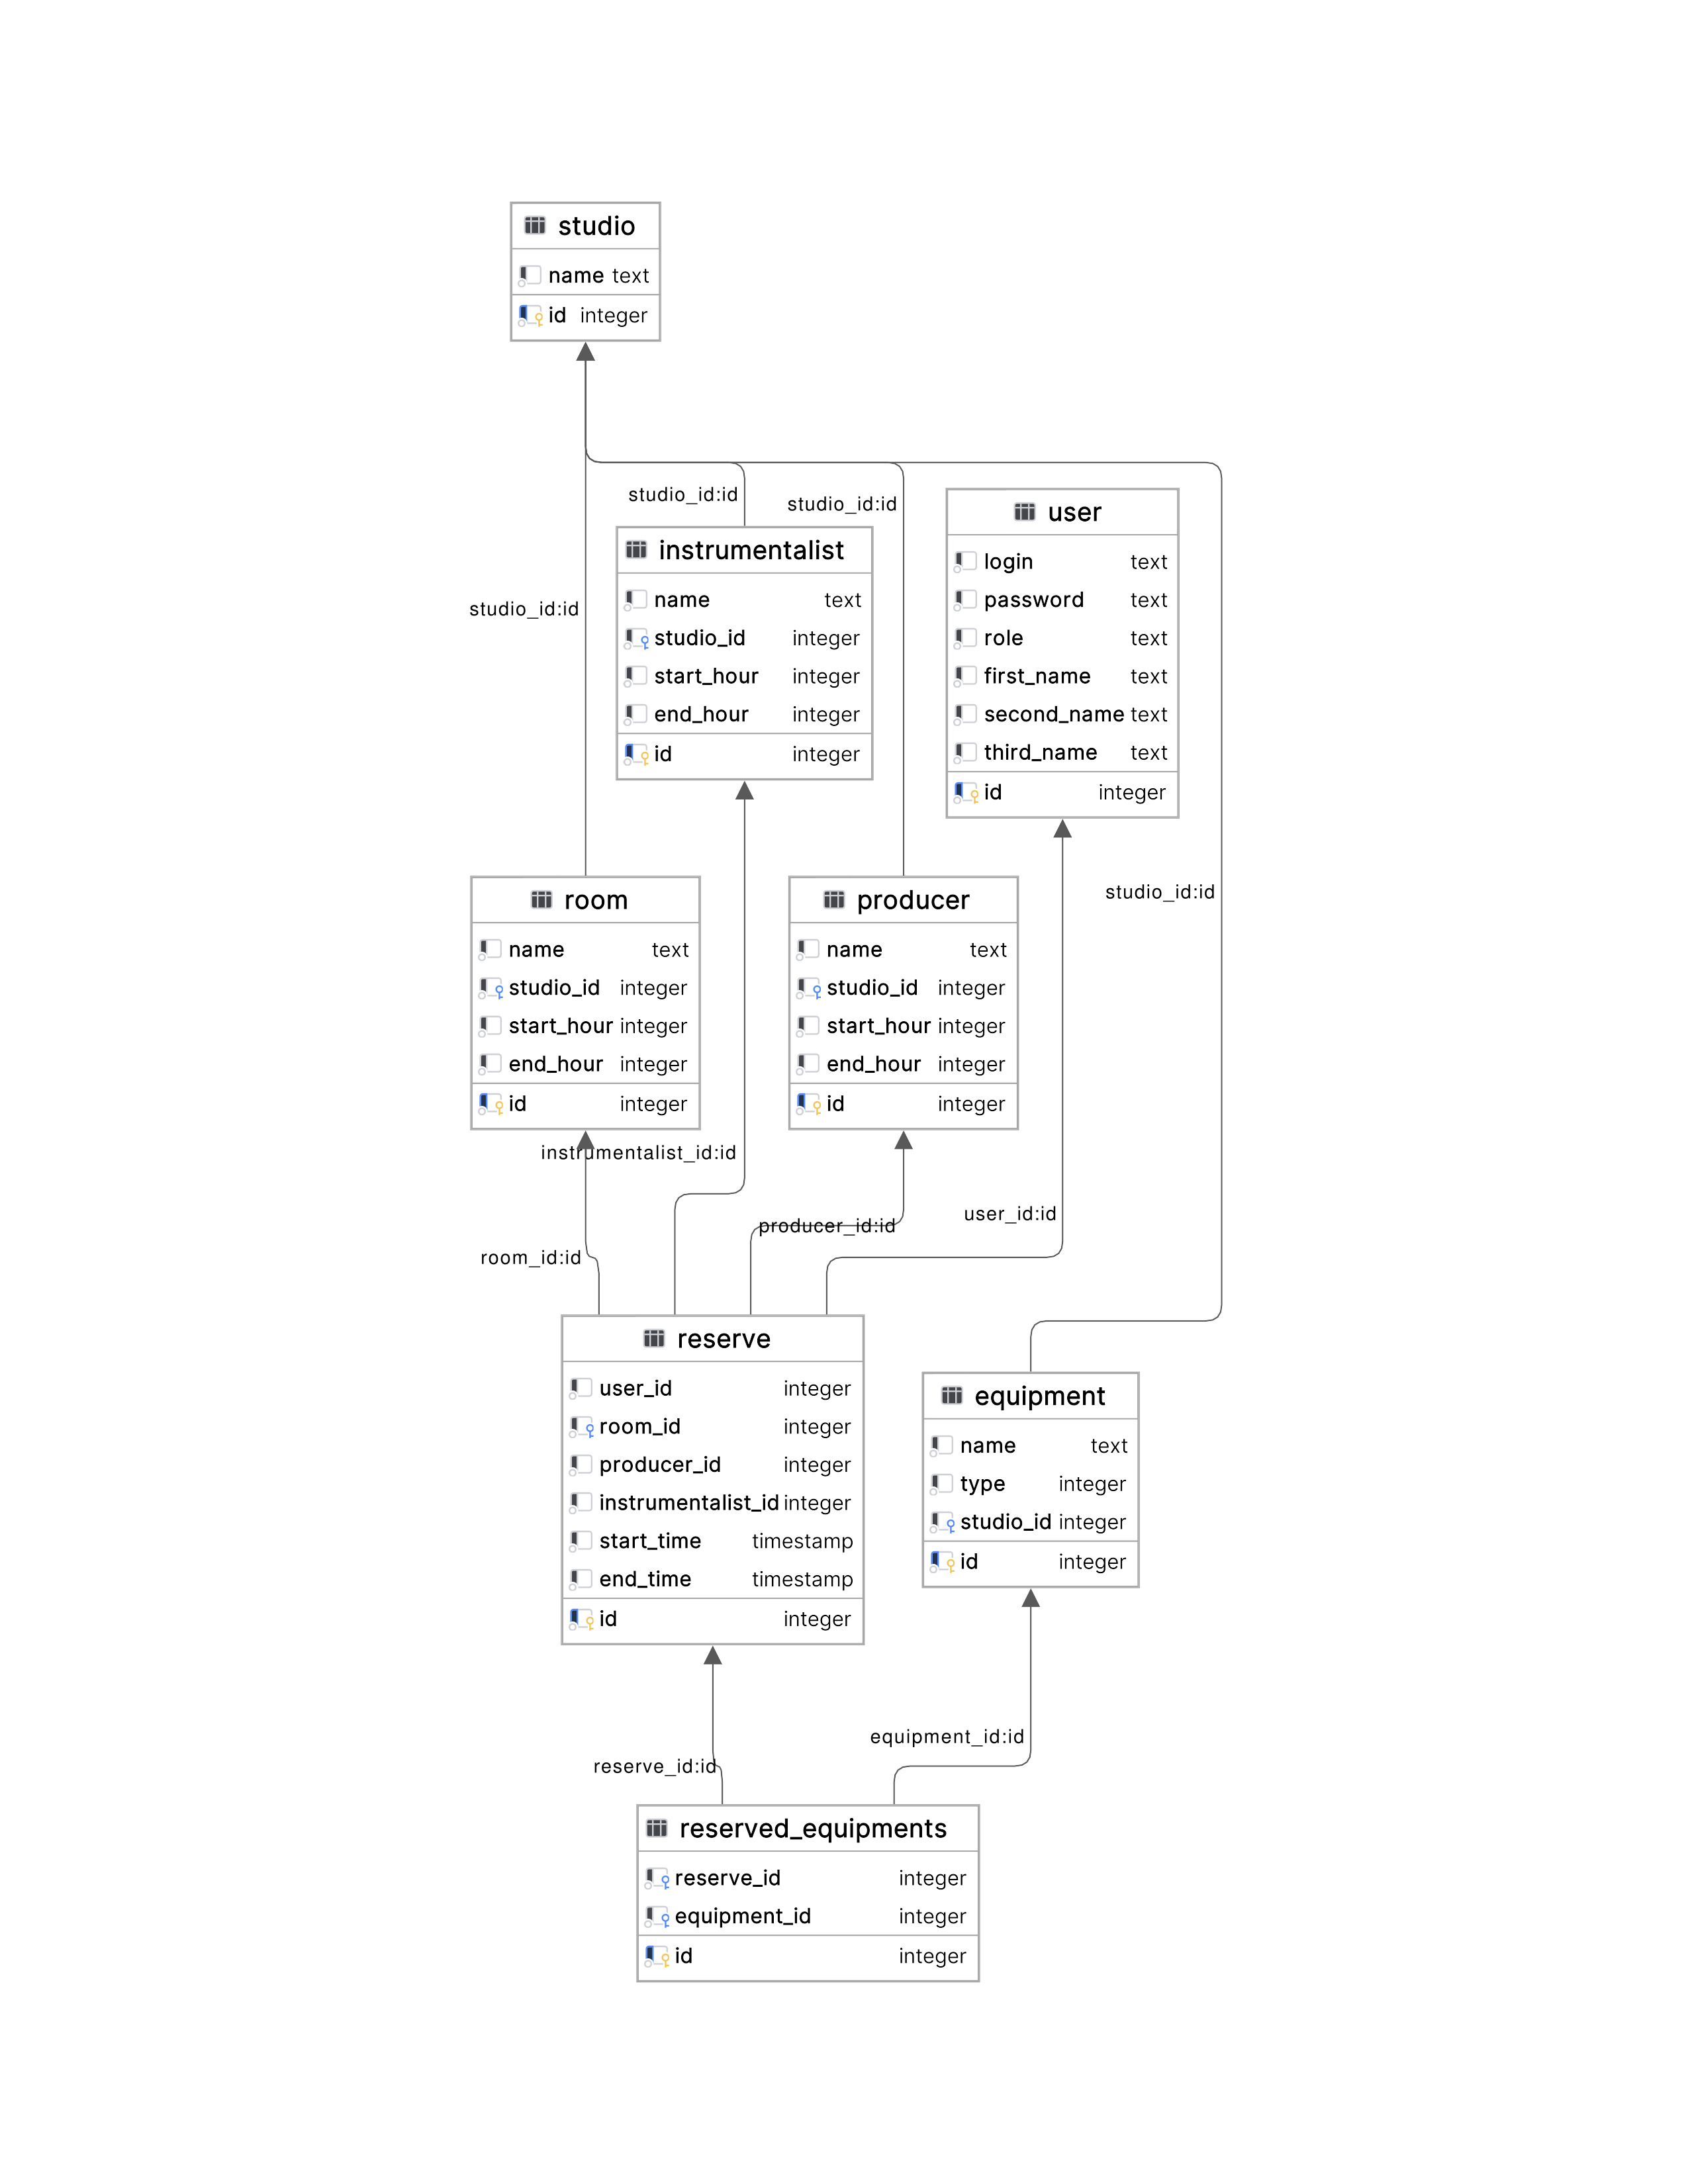
\includegraphics[height=0.83\textheight]{inc/img/public}
%	\captionof{figure}{Диаграмма базы данных}
%	\label{img:db}
%\end{center}

\includeimage
{public} % Имя файла без расширения (файл должен быть расположен в директории inc/img/)
{f} % Обтекание (с обтеканием)
{H} % Положение рисунка (см. wrapfigure из пакета wrapfig)
{0.9\textwidth} % Ширина рисунка
{Диаграмма базы данных} % Подпись рисунка


\section{Описание сущностей}
База данных будет спроектирована из следующих сущностей:
\begin{enumerate}
	\item таблица \textit{User}, в которой хранятся данные об пользователях;
	\item таблица \textit{Reserve}, в которой хранятся данные об бронях;
	\item таблица \textit{Studio}, в которой хранятся данные об студиях;
	\item таблица \textit{Room}, в которой хранятся данные об комнатах студий;
	\item таблица \textit{Equipment}, в которой хранятся данные об оборудовании;
	\item таблица \textit{Reserved\_equipment}, в которой хранятся данные об зарезервированном оборудовании;
	\item таблица \textit{Producer}, в которой хранятся данные об звукорежиссерах студий;
	\item таблица \textit{Instrumentlist}, в которой хранятся данные об инструменталистах студий.
\end{enumerate}
\subsection{Таблица User}
Таблица \textit{User} содержит информацию об идентификаторе пользователя, логине, пароле, роле, имени, фамилии и отчестве.
Имеет следующие атрибуты:
\begin{itemize}
	\item \textit{id} --- целое число, первичный ключ, идентификатор пользователя;
	\item \textit{login} --- строка, логин пользователя;
	\item \textit{password} --- строка, пароль пользователя;
	\item \textit{role} --- целое число, роль пользователя;
	\item \textit{first\_name} --- строка, имя пользователя;
	\item \textit{second\_name} --- строка, фамилия пользователя;
	\item \textit{third\_name} --- строка, отчество пользователя.
\end{itemize}
\subsection{Таблица Reserve}
Таблица \textit{Reserve} содержит информацию об идентификаторе брони, идентификаторе пользователя, идентификаторе комнаты, идентификаторе продюссера, идентификаторе инструменталиста, время начала брони, время конца.
Имеет следующие атрибуты:
\begin{itemize}
	\item \textit{id} --- целое число, первичный ключ, идентификатор брони;
	\item \textit{user\_id} --- целое число, внешний ключ, идентификатор пользователя;
	\item \textit{room\_id} --- целое число, внешний ключ, идентификатор комнаты;
	\item \textit{producer\_id} --- целое число, внешний ключ, идентификатор продюссера;
	\item \textit{instrumentalist\_id} --- целое число, внешний ключ, идентификатор инструменталиста;
	\item \textit{start\_time} --- тип хранения даты и времени, время начала брони;
	\item \textit{end\_time} --- тип хранения даты и времени, время конца брони.
\end{itemize}
\subsection{Таблица Studio}
Таблица \textit{Studio} содержит информацию об идентификаторе студии и названии студии.
Имеет следующие атрибуты:
\begin{itemize}
	\item \textit{id} --- целое число, первичный ключ, идентификатор студии;
	\item \textit{name} --- строка, название студии.
\end{itemize}
\subsection{Таблица Room}
Таблица \textit{Room} содержит информацию об идентификаторе комнаты, названии комнат, идентификаторе студии (к которой принадлежит оборудование), времени начала работы комнаты и времени конца работы комнаты.
Имеет следующие атрибуты:
\begin{itemize}
	\item \textit{id} --- целое число, первичный ключ, идентификатор комнаты;
	\item \textit{name} --- строка, название комнаты;
	\item \textit{studio\_id} --- целое число, внешний ключ, идентификатор студии;
	\item \textit{start\_time} --- тип хранения даты и времени, время начала брони;
	\item \textit{end\_time} --- тип хранения даты и времени, время конца брони.
\end{itemize}
\subsection{Таблица Equipment}
Таблица \textit{Equipment} содержит информацию об идентификаторе оборудования, названии оборудования, типе оборудования, идентификаторе студии (к которой принадлежит оборудование).
Имеет следующие атрибуты:
\begin{itemize}
	\item \textit{id} --- целое число, первичный ключ, идентификатор оборудования;
	\item \textit{name} --- строка, название оборудования;
	\item \textit{type} --- целое число, тип оборудования;
	\item \textit{studio\_id} --- целое число, внешний ключ, идентификатор студии.
\end{itemize}
\subsection{Таблица Reserved\_equipment}
Таблица \textit{Reserved\_equipment} содержит информацию об идентификаторе брони и идентификаторе оборудования (которое принадлежит к брони).
Имеет следующие атрибуты:
\begin{itemize}
	\item \textit{reserve\_id} --- целое число, внешний ключ, идентификатор брони.
	\item \textit{equipment\_id} --- целое число, внешний ключ, идентификатор оборудования.
\end{itemize}
\subsection{Таблица Producer}
Таблица \textit{Producer} содержит информацию об идентификаторе продюссера, имени продюссера, идентификаторе студии (в которой числится продюссер), времени начала работы продюссера и времени конца работы продюссера.
Имеет следующие атрибуты:
\begin{itemize}
	\item \textit{id} --- целое число, первичный ключ, идентификатор продюссера;
	\item \textit{name} --- строка, имя продюссера;
	\item \textit{studio\_id} --- целое число, внешний ключ, идентификатор студии;
	\item \textit{start\_time} --- тип хранения даты и времени, время начала работы продюссера;
	\item \textit{end\_time} --- тип хранения даты и времени, время конца работы продюссера.
\end{itemize}
\subsection{Таблица Instrumentalist}
Таблица \textit{Instrumentalist} содержит информацию об идентификаторе инструменталиста, имени инструменталиста, идентификаторе студии (в которой числится инструменталист), времени начала работы инструменталиста и времени конца работы инструменталиста.
Имеет следующие атрибуты:
\begin{itemize}
	\item \textit{id} --- целое число, первичный ключ, идентификатор инструменталиста;
	\item \textit{name} --- строка, имя инструменталиста;
	\item \textit{studio\_id} --- целое число, внешний ключ, идентификатор студии;
	\item \textit{start\_time} --- тип хранения даты и времени, время начала работы инструменталиста;
	\item \textit{end\_time} --- тип хранения даты и времени, время конца работы инструменталиста.
\end{itemize}

\section{Описание проектируемой ролевой модели на уровне базы данных}
На уровне взаимодействия с БД представлена следующая ролевая модель:
\begin{enumerate}
	\item Guest --- неавторизованный пользователь системы. Имеет права на:
	\begin{itemize}
		\item SELECT, INSERT в таблице User;
		\item SELECT в таблице Reserve.
	\end{itemize}
	\item Client --- авторизованный пользователь системы. Имеет права на:
	\begin{itemize}
		\item SELECT, UPDATE в таблице User;
		\item SELECT, INSERT, DELETE в таблице Reserve;
		\item SELECT, INSERT, DELETE в таблице Reserved\_equipment.
	\end{itemize}
	\item Admin --- администратор системы. Имеет права на:
	\begin{itemize}
	\item SELECT, UPDATE в таблице User;
	\item SELECT, INSERT, UPDATE, DELETE в таблице Studio;
	\item SELECT, INSERT, UPDATE, DELETE в таблице Room;
	\item SELECT, INSERT, UPDATE, DELETE в таблице Producer;
	\item SELECT, INSERT, UPDATE, DELETE в таблице Instrumentalist;
	\item SELECT, INSERT, UPDATE, DELETE в таблице Equipment.
	\end{itemize}
\end{enumerate} 

\section{Описание проектируемых процедур}

На стороне БД, при создании, были определены две процедуры. Обе из них отвечают корректную работу при создании брони.

\subsection{Процедура is\_reserve}
При создании брони запускается процесс транзакции, который включает в себя проверку на занятость выбранных атрибутов (\textit{userId, roomId, producerId, instrumentalistId}) в выбранное время и добавление самой брони.
За проверку занятости отвечает процедура \textit{is\_reserve}, возвращающая булевое значение.
Если ни один атрибут на выбранное время не занят, то возвращается \textit{False}, иначе --- \textit{True}.

На рисунке \ref{img:is_reserve} представлен алгоритм работы проверки занятости.
%\begin{center}
%	\centering
%	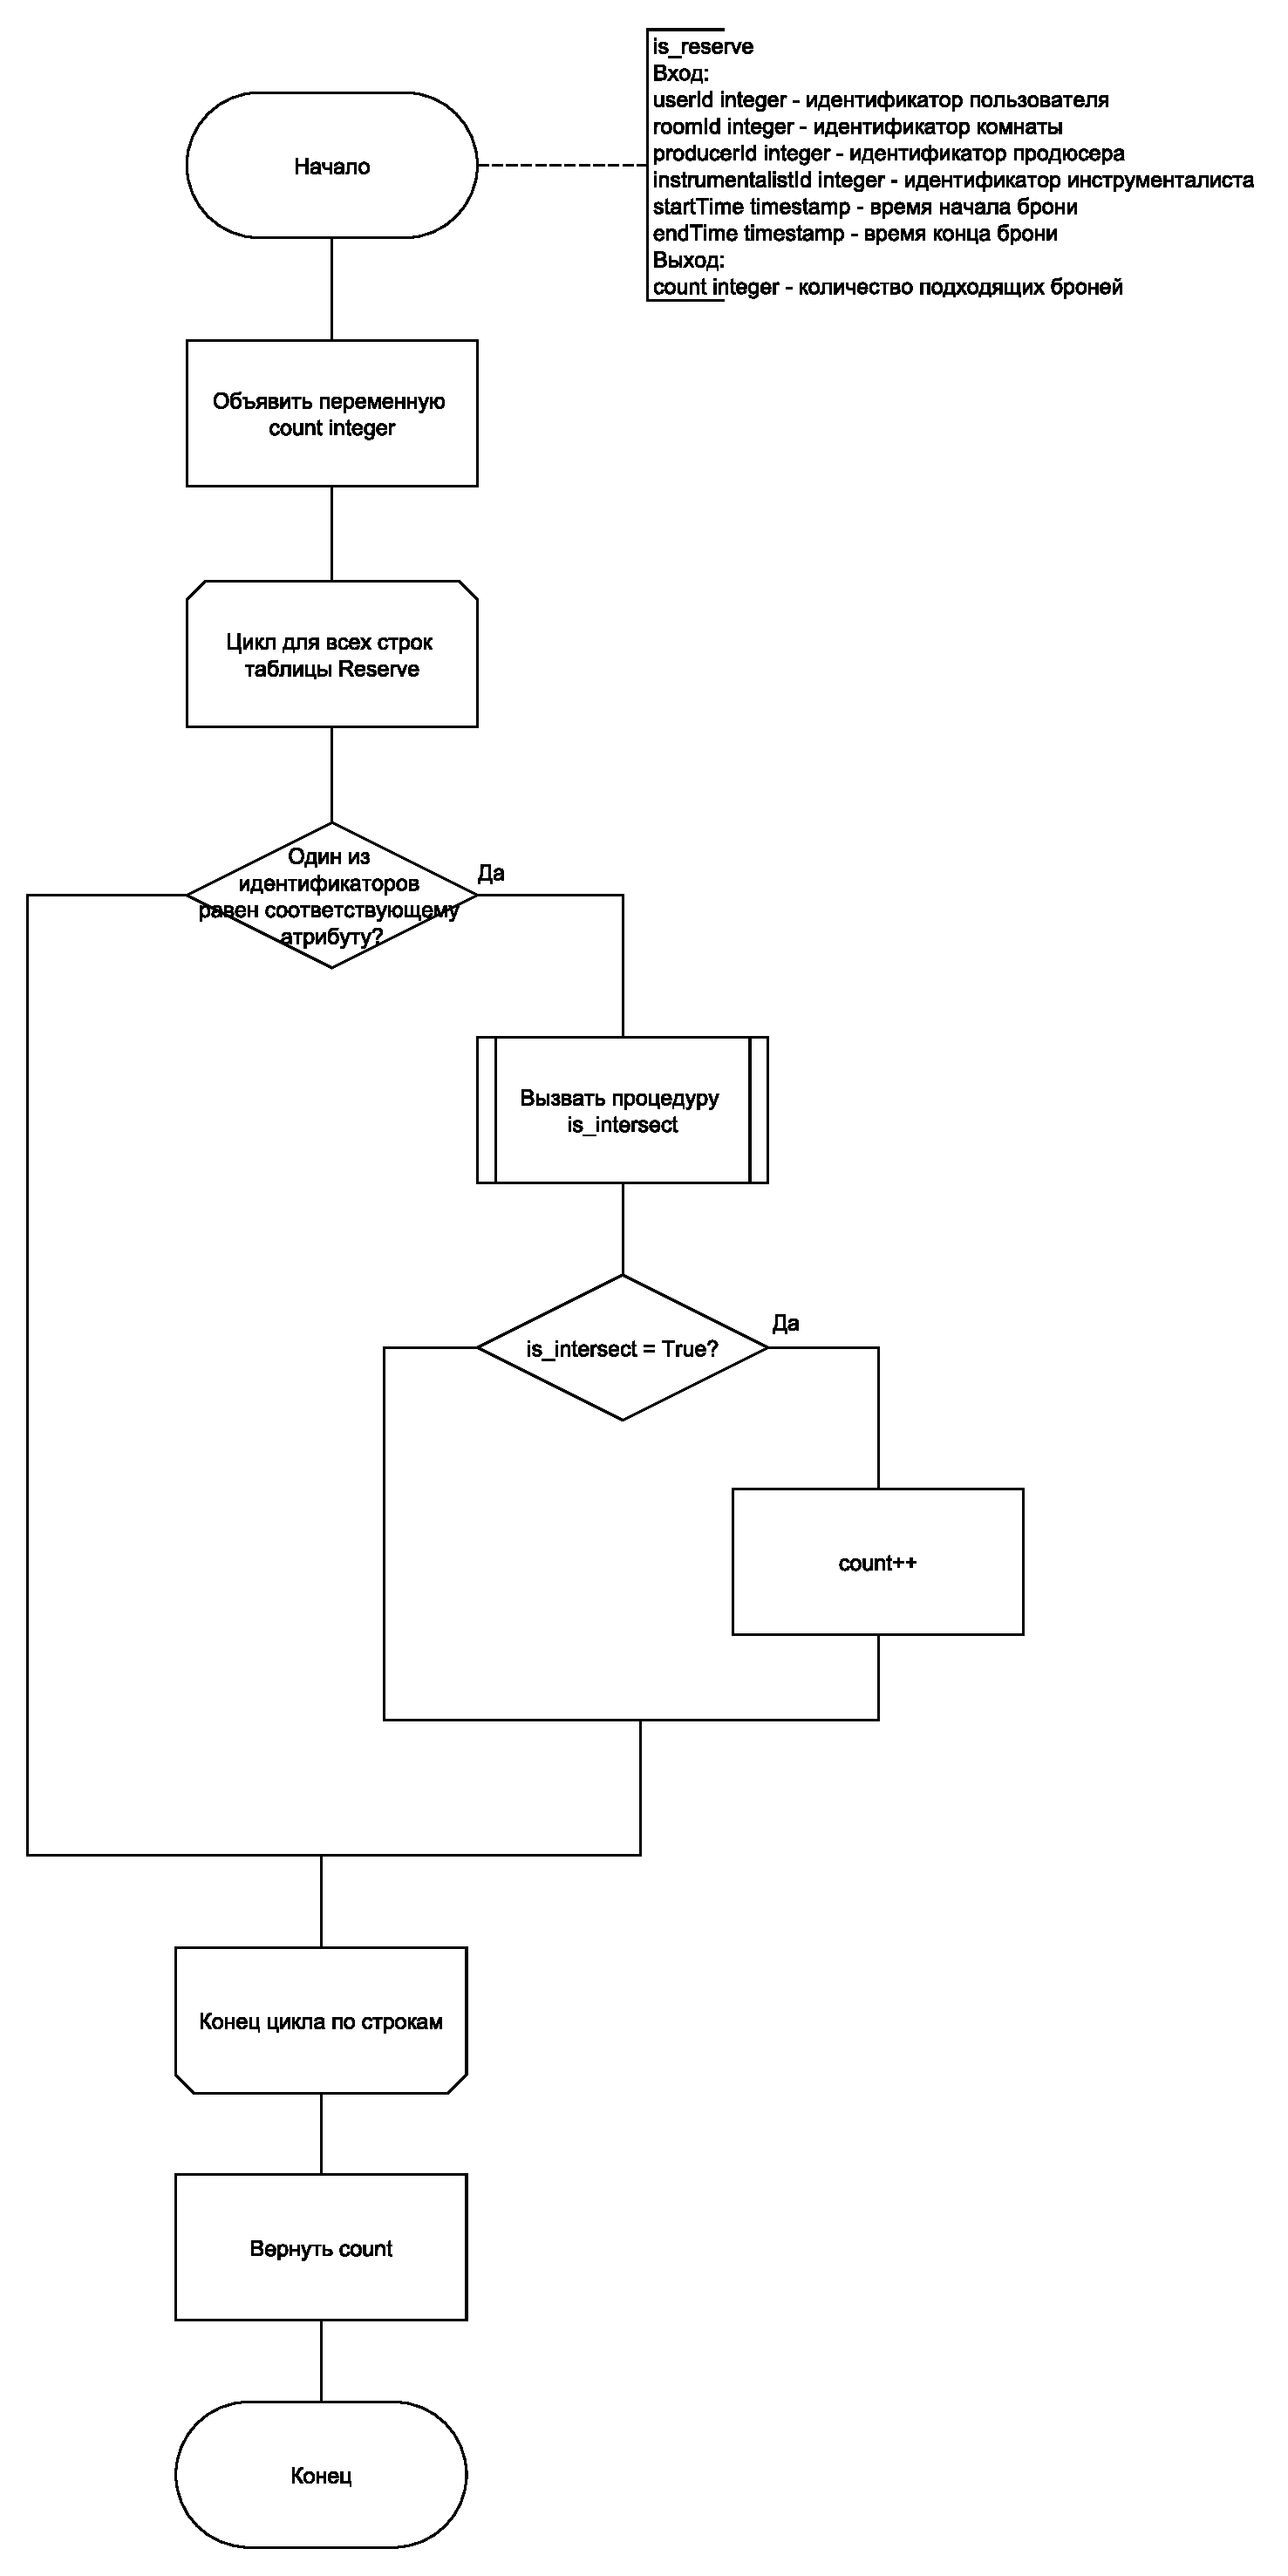
\includegraphics[height=0.95\textheight]{inc/img/is_reserve.pdf}
%	\captionof{figure}{Алгоритм работы проверки занятости}
%	\label{img:is_reserve}
%\end{center}

\includeimage
{is_reserve} % Имя файла без расширения (файл должен быть расположен в директории inc/img/)
{f} % Обтекание (с обтеканием)
{H} % Положение рисунка (см. wrapfigure из пакета wrapfig)
{0.7\textwidth} % Ширина рисунка
{Алгоритм работы проверки занятости} % Подпись рисунка

\subsection{Процедура is\_intersect}
Данная процедура принимает 4 аргумента: выбранное пользователем начало времени, выбранный пользователем конец времени, время начала брони, время конца брони.
Если данные временные отрезки пересекаются, то процедура возвращает True, иначе --- False.

На рисунке \ref{img:is_intersect} представлен алгоритм работы проверки пересечения времени. 
%\begin{center}
%	\centering
%	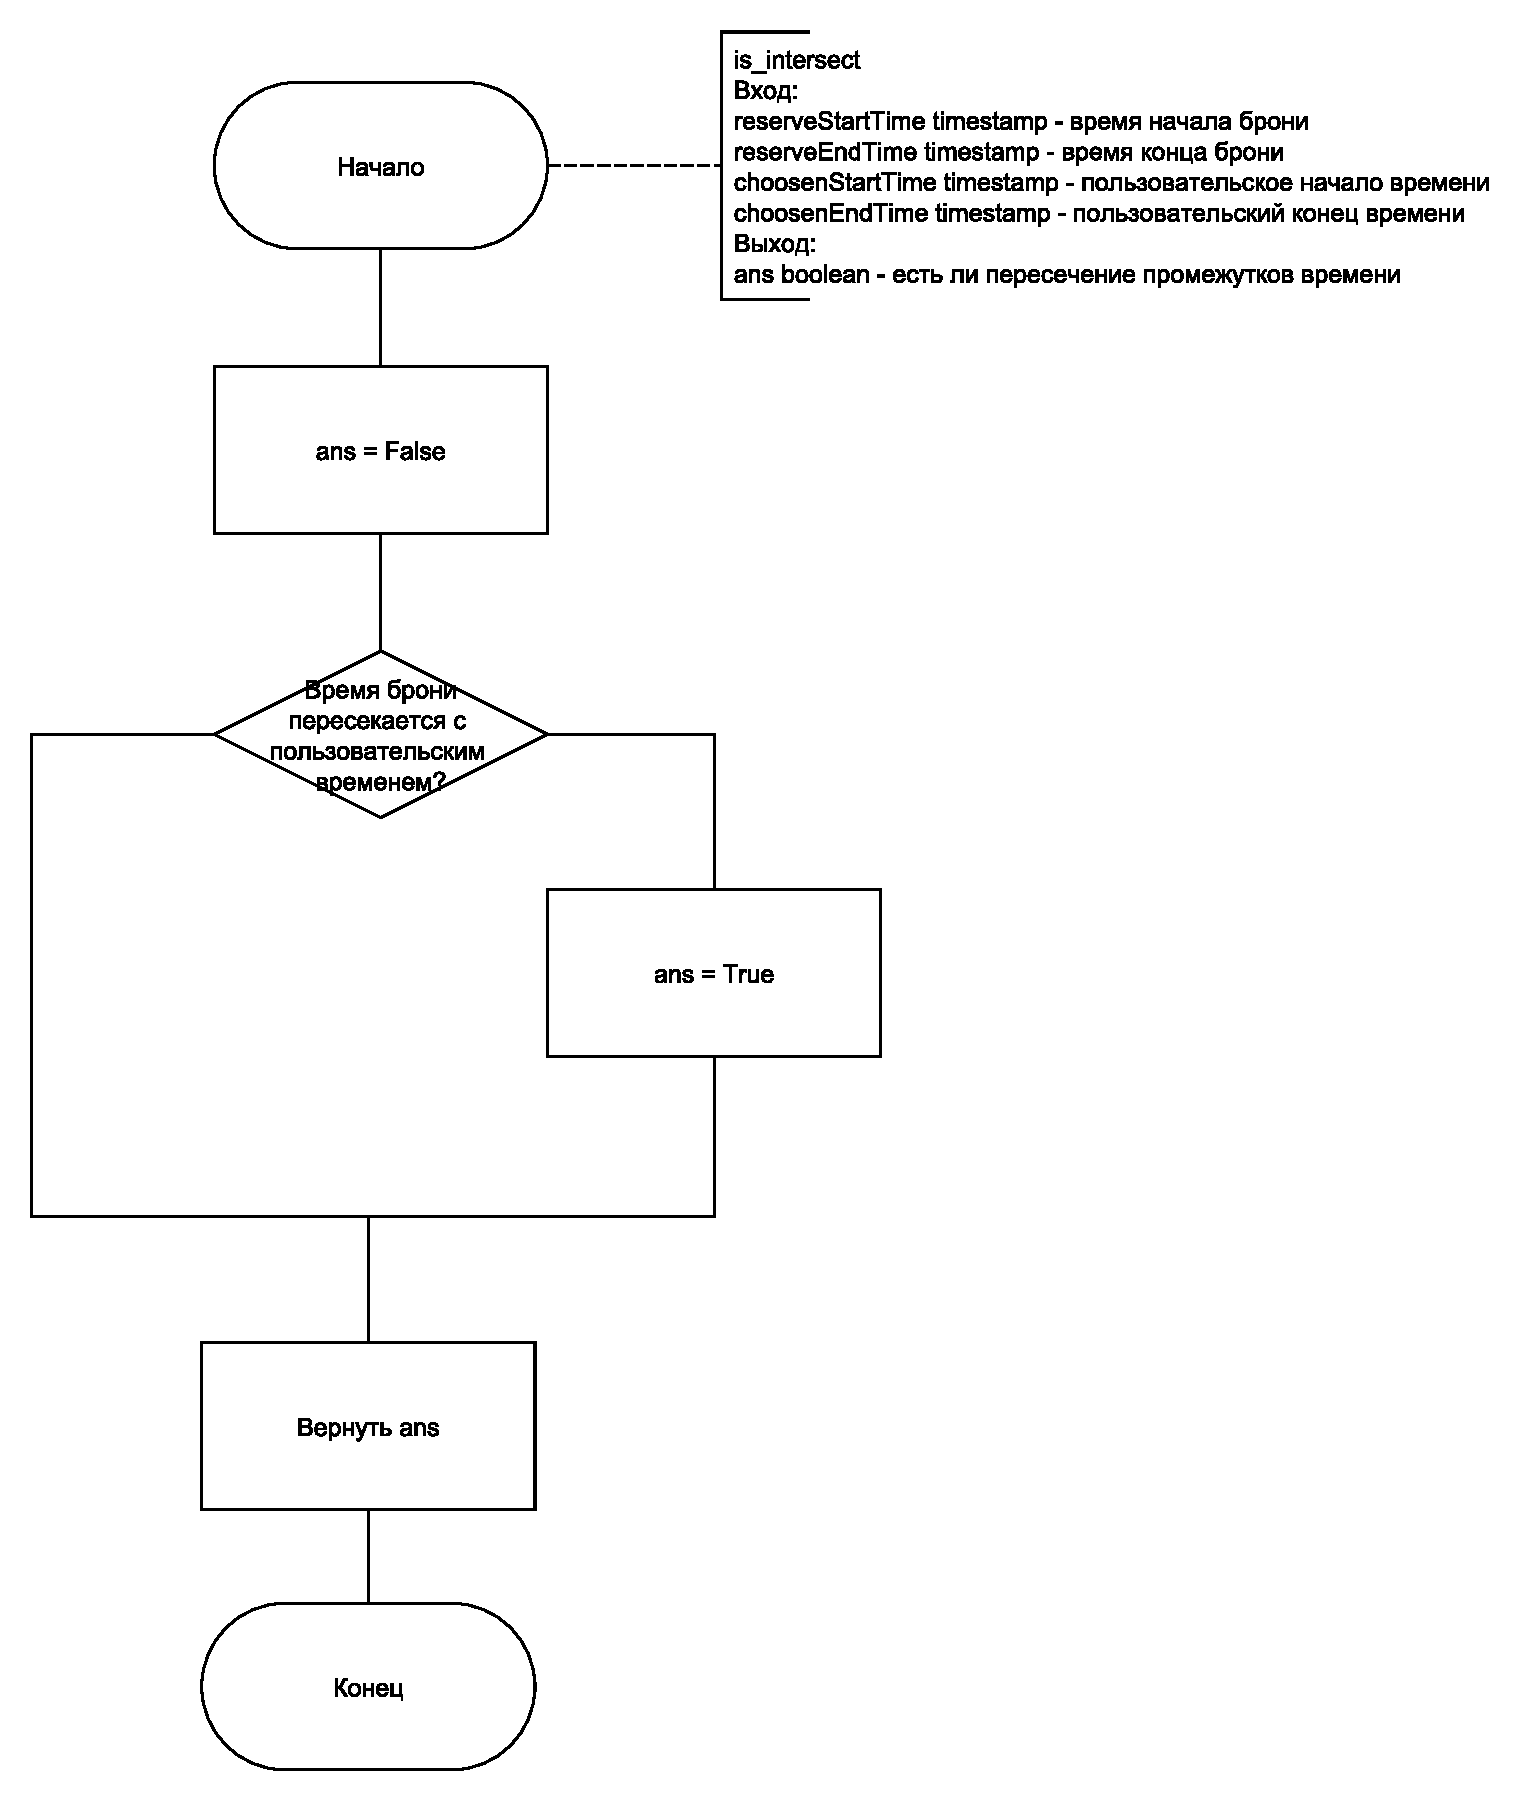
\includegraphics[height=0.65\textheight]{inc/img/is_intersect.pdf}
%	\captionof{figure}{Алгоритм работы проверки пересечения времени}
%	\label{img:is_intersect}
%\end{center}

\includeimage
{is_intersect} % Имя файла без расширения (файл должен быть расположен в директории inc/img/)
{f} % Обтекание (с обтеканием)
{H} % Положение рисунка (см. wrapfigure из пакета wrapfig)
{0.7\textwidth} % Ширина рисунка
{Алгоритм работы проверки пересечения времени} % Подпись рисунка


\section*{Вывод}

В данном разделе была представлена диаграмма проектируемой БД, описание сущностей, описание проектируемой ролевой модели и описание проектируемых процедур.

